\begin{figure}[htb]
\graphicspath{{./figures/}}
    \centering
    \subfloat[] {
        \def\svgwidth{0.5\textwidth}
        \input{figures/trapezoid.pdf_tex}
        \label{fig:segment_trapezoid}
    }
    \hspace{-9em}
    \subfloat[] {
        \def\svgwidth{0.7\textwidth}
        \input{figures/trapezoid_angles.pdf_tex}
        \label{fig:trapezoid_angles}
    }
    \caption{}
    \label{fig:trapezoids}
\end{figure}


\subsection{Cross Section Interval Folding}
\label{sec:interval_folding}

~
\vspace*{-4ex}

\begin{definition}
\label{def:interval}
We consider a cross section composed of segments $ \langle s_1,s_2,\cdots,s_n \rangle$
with total length $X$ (i.e., $\sum \left| s_i\right| = X$).
If we allow this cross section to evolve for time $T$, we obtain a new cross section $\langle r_1,r_2,\cdots ,r_n \rangle$.
The evolution forms a cross section interval $\mathcal C$ of length $T$.
The initial cross section is denoted as $\mathcal C_I = \langle s_1, s_2,\cdots s_n \rangle$,
and the final cross section is denoted as $\mathcal C_F = \langle r_1, r_2,\cdots r_n \rangle$.
\end{definition}

In this section, we focus on a single cross section interval $\mathcal C$ with segments $\langle s_1, s_2,\cdots s_n \rangle$ evolving over time $T$.
First consider the surface traced out by an individual segment $s_i$.
Since the endpoints of $s_i$ move in a straight line, each segment traces a trapezoid.
We define the \emph{height} of a trapezoid to be the distance between its parallel sides.

\begin{lemma}
\label{lem:trapezoid}
The surface traced out by a segment $s$ in time $T$ is a trapezoid $Z_s$ of height $T$ (Figure~\ref{fig:segment_trapezoid}).
Specifically, if $L,R$ are the initial left and right endpoints of $s$, and $L',R'$ are the final endpoints,
$Z_s = LL'R'R$ is the corresponding trapezoid (Figure~\ref{fig:segment_trapezoid}).
\end{lemma}
\begin{proof}
By Invariant~\ref{inv:joint_velocity}, we know that the joint trajectories are straight lines, which form the non-parallel sides.
Since the non-joint nodes on a segment all have the same velocity, the initial and final segment positions form the parallel sides.
\end{proof}

\begin{lemma}
\label{lem:trapezoid_gluing_parallel}
Consider a joint $J$ with segments $l$ and $r$,
which has zero orthogonal joint velocity (i.e., $\vec v_l^\perp = \vec v_r^\perp = \vec 0$).
The gluing of trapezoids $Z_l$ and $Z_r$ along the joint trajectory $\mathcal T_J$ is isometric to a larger trapezoid.
\end{lemma}
\begin{proof}
We consider the evolution of joint $J$ for time $T$ (Figure~\ref{fig:trapezoid_angles}).
First consider a coordinate system with $(\vec{\hat v}_l, \vec{\hat o}_l)$ as the basis.
Since, $\vec{\hat v}_l = \vec v_l^\shortparallel$, from Invariant~\ref{inv:joint_velocity},
we know that $-R_l = \left\| \vec v_l^\shortparallel\right\|\cdot\cot(\omega) = \cot(\omega)$.
So, $\vec J_v = \vec{\hat v}_l - \vec{\hat o}_v\cdot\cot(\omega)$.  Therefore,
\begin{align*}
    \cot(\angle LJJ') &= \frac{T\cdot R_l}{ \left\| T\cdot\vec{\hat v}_l\right\|} = \cot(\omega)
    \implies \angle LJJ' = \omega.
\end{align*}
Similarly, we consider a coordinate system with $(\vec{\hat v}_r, \vec{\hat o}_r)$ as the basis.
Since $\vec J_v = \vec{\hat v}_r - \vec{\hat o}_r\cdot \cot(\omega)$, we get
$$
\cot(\angle RJJ') = \frac{-\left\| T\cdot L_r\right\|}{ \left\| T\cdot(\vec J_v - L_r)\right\|} = -\cot(\omega)
\implies \angle RJJ' = \pi - \omega.
$$
This implies that $\cot(\angle RJJ') + \cot(\angle LJJ') = \pi$.
So, the gluing of $Z_l$ and $Z_r$ along the joint trajectory $JJ'$ is isometric to a larger trapezoid.
\end{proof}

\begin{figure}[!htb]
\graphicspath{{figures/trapezoidZ}}
    \centering
    %\subfloat[]{
        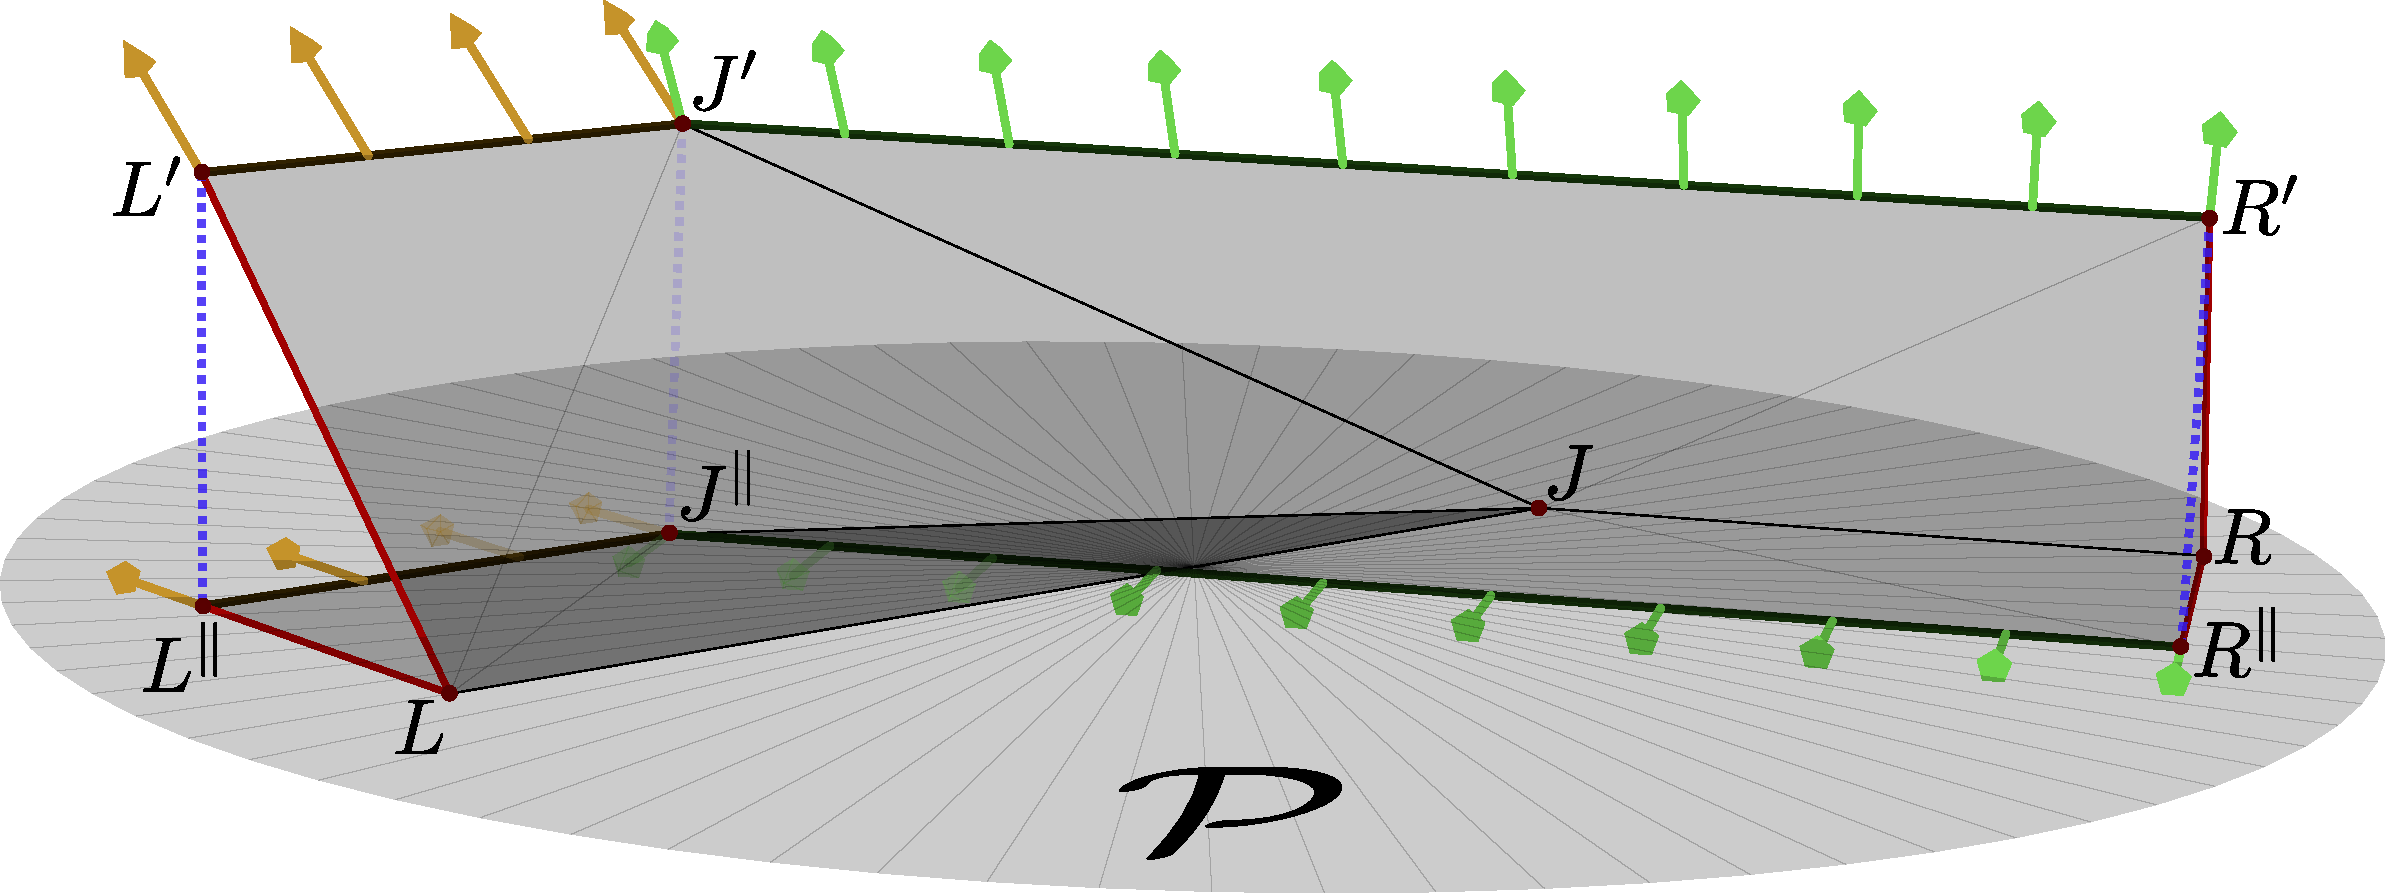
\includegraphics[width=0.5\textwidth]{figures/trapezoidZ/trapezoidZ0.pdf}%
    %}%
    %\subfloat[]{
        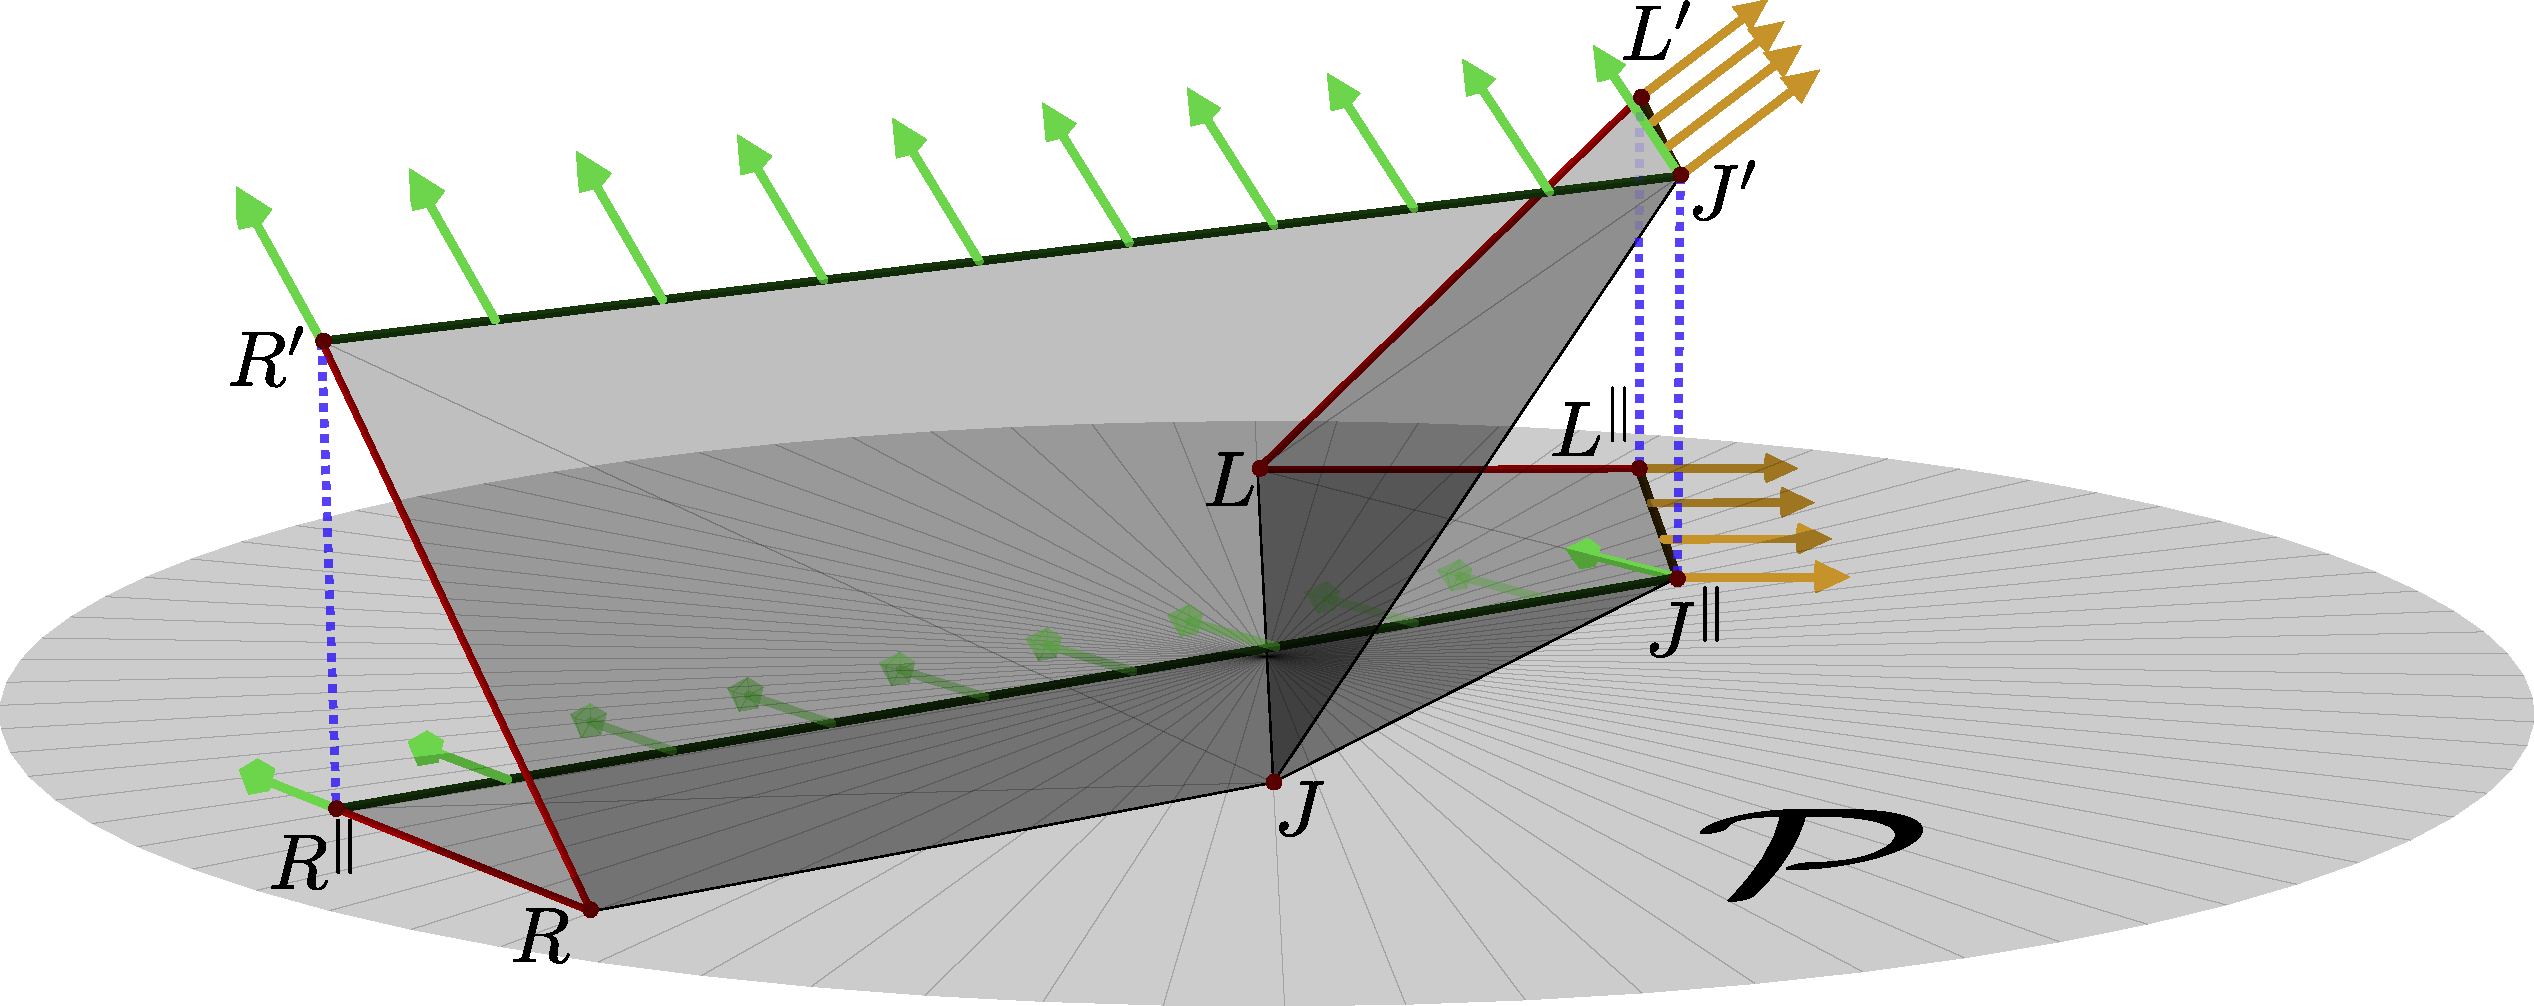
\includegraphics[width=0.5\textwidth]{figures/trapezoidZ/trapezoidZ1.pdf}%
    %}%

    %\subfloat[]{
        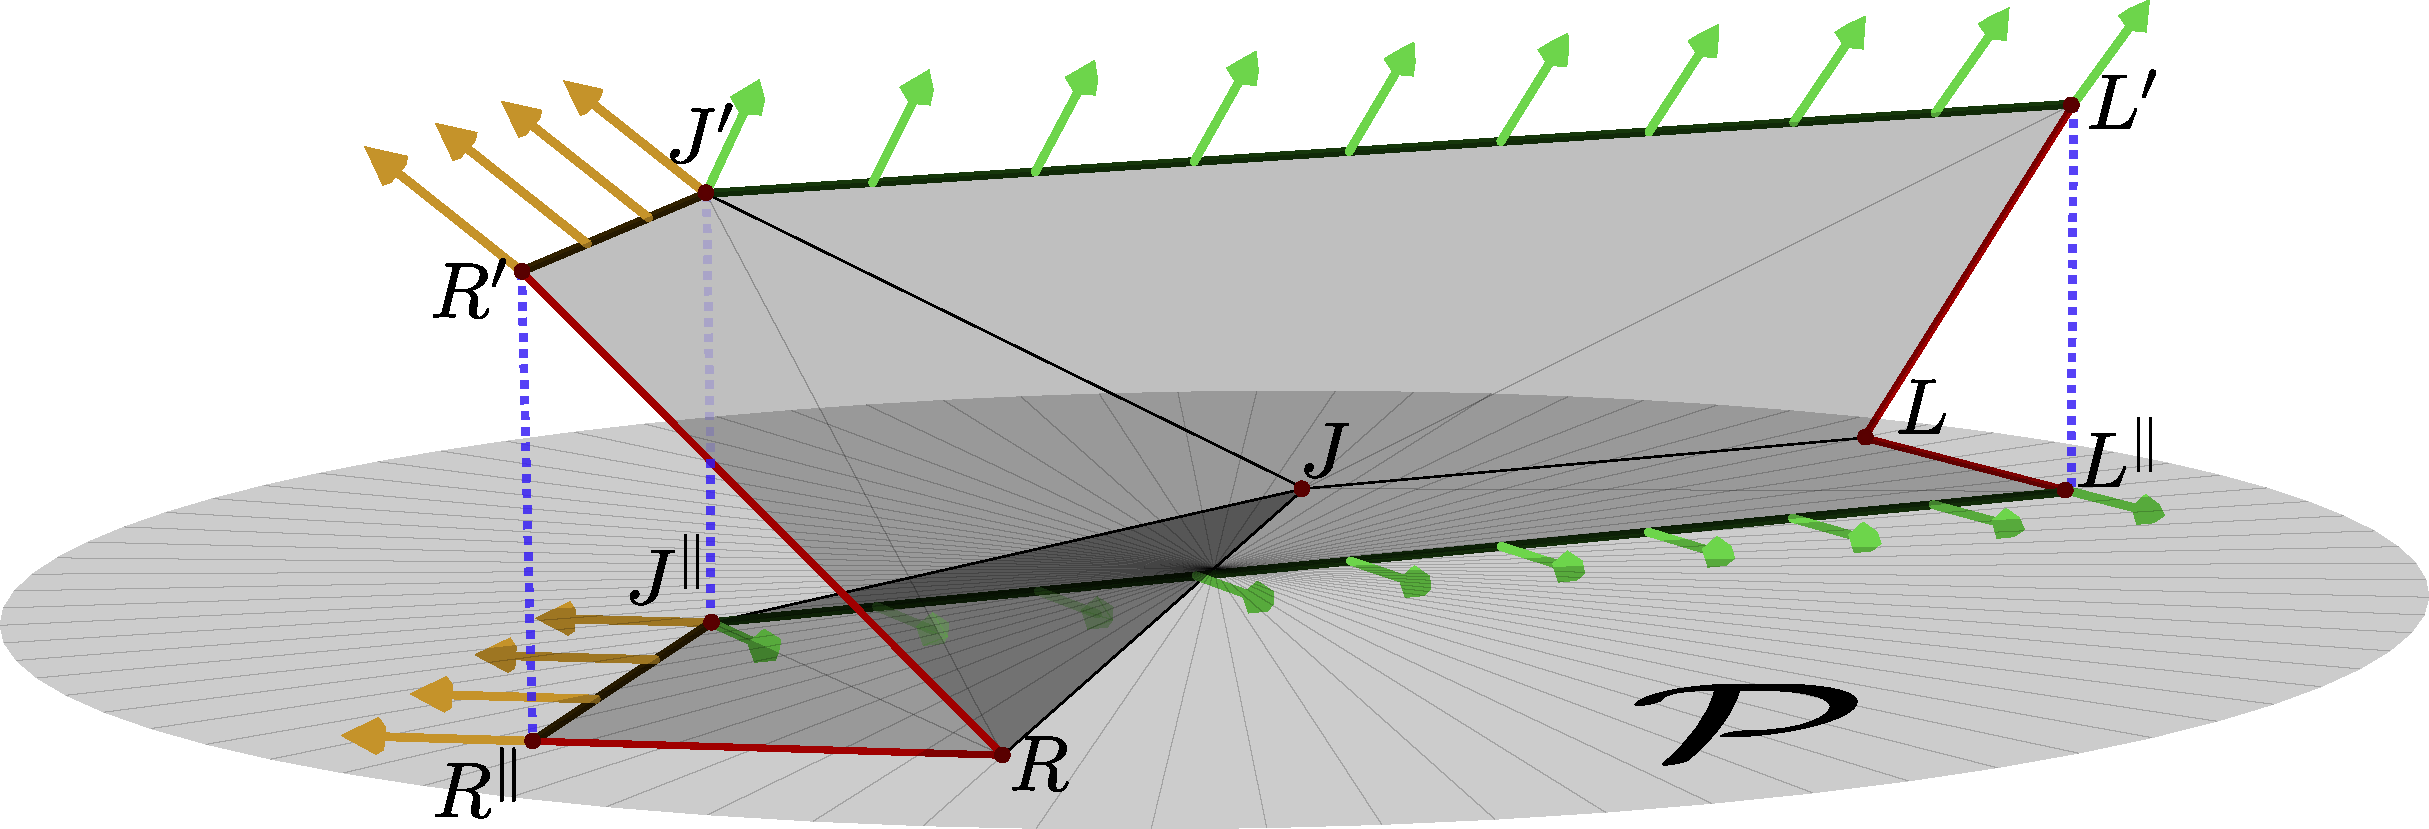
\includegraphics[width=0.8\textwidth]{figures/trapezoidZ/trapezoidZ2.pdf}%
    %}%
    \caption{
    Evolution of a joint with non-zero orthogonal velocity from $LJR$ to $L'J'R'$.
    The blue dotted lines represent the projection of the final state to the joint plane $\mathcal P$.
    }
    \label{fig:trapezoidZ}
\end{figure}


~
\vspace*{-4ex}

\begin{lemma}
\label{lem:trapezoid_gluing}
Consider a joint $J$ with segments $l$ and $r$ with non-zero orthogonal velocity; see Figure~\ref{fig:trapezoidZ}.
The gluing of trapezoids $Z_l$ and $Z_r$ along the joint trajectory $\mathcal T_J$ is isometric to a larger trapezoid.
\end{lemma}

\begin{proof}
As before, let $LJR$ and $L'J'R'$ represent the initial and final positions of the segments respectively.
We also construct the projection of $L'J'R'$ to the joint plane $\mathcal P$ as $L^\shortparallel J^\shortparallel R^\shortparallel$.
The evolution of the projection is analogous to the setting in Lemma~\ref{lem:trapezoid_gluing_parallel}.
Therefore, $\angle LJJ^\shortparallel = \omega = \theta/2$ and $\angle RJJ^\shortparallel = \pi-\omega$.

Consider the positive $z$-axis along the joint orthogonal velocity (i.e., normal to the joint plane $\mathcal P$).
We define the orthogonal displacement vector as $\overrightarrow{JJ'} = z\cdot\vec{\hat k}$.
Let the positive $x$-axis be along $JJ^\shortparallel$. So, the unit vector along $\overrightarrow{JJ'}$ is $\frac{1}{\sqrt{1+z^2}}(1,0,z)$.

Since $\angle J^\shortparallel JR = \omega$, the unit vector along $\overrightarrow JR$ is $(\cos\omega,\sin\omega,0)$.
So, we compute $\cos \angle RJJ' = \cos\omega/\sqrt{1+z^2}$.
Similarly, since $\angle J^\shortparallel JL = \pi-\omega$, the unit vector along $\overrightarrow JL$ is $(-\cos\omega,\sin\omega,0)$,
which implies that $\cos \angle LJJ' = -\cos\omega/\sqrt{1+z^2}$.
Finally, since both $\angle LJJ$ and $\angle RJJ'$ are less than $\pi$, and $\cos\left(\angle LJJ' \right) = -\cos\left(\angle RJJ' \right)$,
we conclude that $\angle LJJ' + \angle RJJ' = \pi$.
Since $LJJ'L'$ and $RJJ'R'$ are both trapezoids, this implies that the resulting gluing along $JJ'$ is isometric to a larger trapezoid.
\end{proof}

\begin{definition}
\label{def:interval_folding}
Consider a cross section interval $\mathcal C$ formed from a cross section $C$ evolving over time $T$.
By Lemma~\ref{lem:trapezoid}, the segments $ \langle s_1, s_2,\cdots s_n \rangle$ form trapezoids
$ \langle Z_1, Z_2,\cdots Z_n \rangle$ each of height $T$, where $Z_i$ represents the $i^{th}$ trapezoid in folded space.
The folding (the final folded state) $\mathcal F_C^T$ corresponding to $\mathcal C$ is formed by successively gluing the trapezoids
$Z_i$ to $Z_{i+1}$ along the trajectory of joint $\vec J_i$ (for $1\le i<n$) to form a connected shape.
\end{definition}

\begin{definition}
\label{def:interval_folding_boundary}
Given a cross section interval $\mathcal C$ with folding $\mathcal F_C^T$,
the initial-boundary of a folding $\mathcal F_C^T$ is defined as the union of the initial cross section segments in $\mathcal C_I$,
where the right endpoint of the $i$th segment is attached to the left endpoint of the $(i+1)$st segment.
Similarly, the final-boundary of $\mathcal F_C^T$ is defined as the union of the final segments in $\mathcal C_F$.
\end{definition}

\begin{restatable}{thm}{interval_strip}
\label{thm:interval_strip}
Consider a cross section interval $\mathcal C$ formed from a cross section $C$ evolving over time $T$ to form a folding $\mathcal F_C^T$.
Further assume that the total length of cross section $C$ is $X$ units. Then, $\mathcal F_C^T$ is isometric to a $X\times T$ strip of paper.
\end{restatable}
\begin{proof}
By repeated use of Lemma~\ref{lem:trapezoid_gluing}, we know that $\mathcal F_C^T$ is isometric to a trapezoid.
Let $L,L'$ be the initial and final positions of the left (non-parallel) edge of the trapezoid, and
let $R,R'$ be the initial and final positions of the right edge of the trapezoid.
Say that $C$ comprises of segments $ \langle s_1, s_2,\cdots s_n \rangle$.
From Invariant~\ref{inv:left_right_pace}, we know that the left pace of $s_0$ is zero.
So, the line $LL'$ follows the trajectory of $\vec{\hat v_0}$, which is orthogonal to the segment $s_0$.
In other words, the left edge of the trapezoid has length $T$, and is orthogonal to the parallel edges.
Similarly, because the right pace of $s_n$ is zero, the right edge of the trapezoid is also orthogonal.
Therefore, $\mathcal F_C^T$ is isometric to a right angled trapezoid (i.e., a strip) of length $X$ and width $T$.
\end{proof}

\begin{remark}
\label{rem:joint_crease}
The trajectory of a joint forms a crease in the folded state.
\end{remark}
